\documentclass{article}
%
\usepackage[mathcal,mathbf]{euler}
%\usepackage{theorem,amsmath,enumerate,fancyhdr,amssymb,accents,amsfonts}
\usepackage{theorem,amsmath,enumerate,fancyhdr,amssymb,amsfonts}
\usepackage[pdftex]{graphicx}
%% In order to be consistent use the notation in the following style
%% file as much as you can. You may take a look at the file to see
%% what is available.
\usepackage{myDefs}
\usepackage{undertilde}

%%
%% Here is where the title goes. Write down lecture number for ?
\title{ 
Algorithmic Learning Theory\\
Spring 2017\\
Lecture 3 %1 or 2 or 3 etc
}
\author{
{\bf Instructor:} Farid Alizadeh\\
{\bf Scribe:} Atharv Bhosekar
}
\date{02/01/2017} %put the date of the lecture here NOT the date the note was written

\begin{document}

\pagestyle{fancy}
\lhead{{\bf scribe:}{Atharv Bhosekar}
\\{\bf Lecture 3} } %insert lecture number
\rhead{{\bf Date: }02/01/2017} %enter lecture date NOT today's date

\maketitle
%
\oddsidemargin 0.0in 
\textwidth 6.25in 
\topmargin -0.25in 
\textheight 8.25in    

%%%%%%%%%%%%%%%%%%%%%%%%%%%%%%%%%%%%%%%%%%%%%%%%%%%%%%%%%%%%%%
%% Below  is where the body of your notes goes.
%%%%%%%%%%%%%%%%%%%%%%%%%%%%%%%%%%%%%%%%%%%%%%%%%%%%%%%%%%%%%%

%%\begin{document}   
\medskip

%% Write a quick short paragraph summarizing the topic covered in
%% the lecture here. You may use itemization or enumeration
This document introduces k-Nearest Neighbor (k-NN) method and discusses the following:  
\begin{enumerate}
\item k-NN overview 
\item k-NN for regression
\item key features of k-NN
\item notion of nearness
\item voronoi diagrams
\item computational complexity of k-NN
\item Issue with high number of features
%etc
\end{enumerate}

\section{Overview} %give a one paragraph short description of the topics
k-NN as the name suggests, takes k nearest points in the available data set to the desired new point, averages the responses for those points and reports that as the response at the new point. To better visualize this, consider an example of a classification problem with two features denoted by $x_1$ and $x_2$ and two classes denoted by blue and black color as shown in Figure \ref{Fig.1}. The problem is to classify the new point (the point denoted in red color) as blue or black. For illustration, consider $k = 3$ i.e. consider three nearest neighbors to the new point. Three points shown in the circle are found to be closest to the new point and two of these neighboring points are blue and one is black. Taking average of three points, the new point is 2/3rd likely to be blue and 1/3rd likely to be black. Therefore,the k-NN algorithm classifies the new point as blue. One small point to notice here is that the class reported based on k-NN is the class that has maximum value and does not take in to consideration the magnitude by which that class is favored over the other class.

Relating this concept to the Bayes' decision rule, with a vector of features $\utilde{x} = (x_1, x_2, \dots, x_p)$ where $p$ is the number of features. The problem is to find $Y_{\mathrm{new}} = \underset{y}{\mathrm{argmax}}\, Pr[Y|\, \utilde{x}_{\mathrm{new}}]$. To put it in words, given a new point $x$ the problem is to find the probability that it belongs to class black or blue or any other class name relevant to the problem. The problem however is that we have no information about the probability.
\begin{figure}
\begin{center}
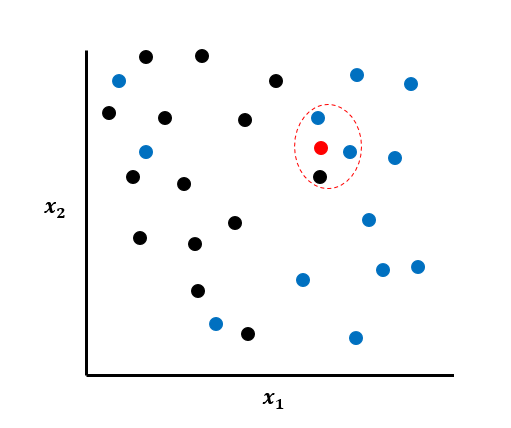
\includegraphics[scale=0.5]{classificationkNN.PNG}
\caption{Example of a 2 feature 2 class classification problem. Red point shows the point to be classified. Points in the red dotted circle denote 3 nearest neighbors.}
\label{Fig.1}
\end{center}
\end{figure}
k-NN solves this problem by implicitly making two assumptions. First, it replaces $x_{\mathrm{new}}$ with k- neighbors of $x_{\mathrm{new}}$. Second, it approximates probability of the entire population by sample proportion which is said to be approximately equal to the proportion in the neighborhood of each class.



\section{k-NN for regression}
Similar to classification, k-NN for regression is analogous to Bayes' decision rule for regression. Looking back at classification, the classification rule is obtained by minimizing loss function that quantifies misclassification. In case of regression, usually the loss function is defined as $\mathrm{loss}(x, \hat{f}|\,f) = (f(x) - \hat{f}(x))^2$ which is sum of squared errors. Our aim is to minimize the expected loss given by $\mathrm{risk}(\hat{f}|\,f) = \mathbb{E}_x(f(x) - \hat{f}(x))^2$. Assuming we have the entire population, best $\hat{f}$ is given by $\hat{f} = \mathbb{E}_x(y)$, which is the average of all possible values of $y$.
Two assumptions that k-NN makes implicitly for the case of classification are made even for the case of regression. For example, $x_{\mathrm{new}}$ is replaced by k closest data points $x_i$ and average of all $y$ responses at $x_{\mathrm{new}}$ are approximated by responses at k nearest neighbors.

\section{Key features of k-NN}
k-NN is a purely non-parametric method. This can be derived from the observation that the loss function in case of both classification as well as regression does not make any assumption on the nature of surrogate function $\hat{f}$.

\subsection{Notion of nearness}
Entire k-NN method is dependent on finding and utilizing k-nearest neighbors. However, there are some issues that one needs to take in to account while defining nearness. 

It is important to note that the operation on the responses of $k$ nearest neighbors to obtain the response at a new point is dependent on the loss function. For example, average is used only if the loss function is squared error, median will be used if the loss function is sum of absolute values and so on.

\subsubsection{Definition of distance}
First, notion of nearness is most of the times problem dependent based on the definition of distance. There are number of different ways to define distance between two distinct data points. The most common distance used for numerical problems (classification and regression involving numbers) is Euclidean distance which is defined as $\| \utilde{a} - \utilde{b}\| = \sqrt{(a_1 - b_1)^2 + (a_2 - b_2)^2 +\dots{•}+ (a_p - b_p)^2}$. There are some other types of distances that one might encounter. For example, $l_1$ distance = $\| \utilde{a} - \utilde{b} \|_1$ = $\|a_1 - b_1\| + \dots{.} + \|a_p - b_p\|$. In general, $l_r$ distance is given by $[(a_1 - b_1)^r + \dots{} + (a_p - b_p)^r]^{1/r}$. Two more special cases of this general form that are used often are $l_{\infty} = \max{|a_i - b_i|}$ and $l_0$ that signifies number of items that are not equal (or classified incorrectly). If individual features are not useful then one can also define distance as $|X - Y|$ = 0 if $X$ and $Y$ are same from class and $|X - Y|$ = 1 if $X$ and $Y$ are from different classes. If the problem is not numerical (say words) then an example distance metric can be hanning distance $|"a_1a_2\dots{}a_n" - "b_1b_2\dots{}b_n"|$.

\subsubsection{Scale dependence}
Second issue arises from the scale dependence of distance irrespective of the way we define distance. To illustrate this, a simple example of three points is considered. Given three data points as follows:
$a$ = (45, \$76000), $b$ = (25, \$75000), $c$ = (42, \$78000). Distance between points $a$ and $b$ can be written as $\mathrm{d}(a, b) = \|a - b\| = \sqrt{\mathrm{20^2} + \mathrm{1000^2}} \approx$ 1000. Similarly, $\mathrm{d}(b,c) \approx$ 3000 and $\mathrm{d}(a,c) \approx$ 2000. Changing the scale of second co-ordinate by a factor of 1000, one can write the same distance as $\mathrm{d}(a, b) = \|a - b\| = \sqrt{\mathrm{20}^2 + \mathrm{1}^2} \approx$ 20, $\mathrm{d}(b,c) \approx$ 17 and $\mathrm{d}(a, c) \approx$ 3.6. As it can be seen clearly, that by changing the scale, now $c$ is closer to $a$ than $b$ unlike the previous case. Thus, scale in which data is reported can affect selection of nearest points and this makes outcome of k-NN scale dependent. 

There are solutions to avoid issues with scale dependence such as standardizing the data and it is important to get a brief idea about how it can be helpful. Assuming that the data roughly follows a normal distribution we transform data $\utilde{x} \rightarrow X_1, X_2,\dots{.},X_N$ to obtain a standardized data using $X_k = \frac{X_1 - \bar{X}}{s}$ where $\bar{X} = \frac{X_1 + X_2 + \dots{.} + X_N}{N}$ which is mean and $s = \frac{\sqrt{(X_1 - \bar{X})^2 + \dots{.} + (X_N - \bar{X})^2}}{N-1}$ which is standard deviation. One point notice in case of this standardization is that this approach is effective only when features are completely independent of each other. If the features are correlated, one might end up overemphasizing some of the features and under-emphasizing some. To avoid this, use of a covariance matrix is suggested. Covariance matrix $\mathbb{S}$ is defined as $\mathbb{S}_{ij} = \sum_l(x_{il} - \bar{x_i})(x_{jl} - \bar{x_j})$. This implies that $X_i \rightarrow (X_i - \bar{X}1)^T\mathbb{S}^{-1} (X_i - \bar{X}1)$. Therefore, $d(a, b) = \sqrt{(a - b)^T \mathbb{S}^{-1}(a - b)}$. To put it simply, if the correlation is large intuitively, $\mathbb{S}^{-1}$ becomes small and it weighs down the distance. As a result of these computations, evaluating $\hat{f}$ at a new point is expensive.

\section{Voronoi diagrams}
Voronoi diagrams use the principle of k-NN in the sense that it divides the space based on the nearest sample (or one nearest neighbor) of point. For example, if one has two data points in the space, the space is divided in to two halfspaces from the mid-point of those two data points. Similarly, k-level voronoi diagrams use the principle of k nearest neighbors. A sample Voronoi diagram is shown in Figure \ref{Fig.2}.
\begin{figure}
\begin{center}
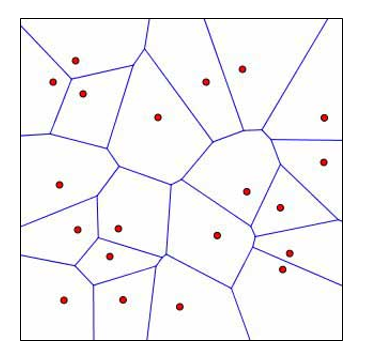
\includegraphics[scale=0.5]{voronoiExample.PNG}
\caption{Voronoi diagram example}
\label{Fig.2}
\end{center}
\end{figure}

\section{Computational complexity of k-NN}
Using efficient data structures such as a binary search tree to find the nearest neighbors, it can be shown that the computational efforts involved are proportional to depth of the tree which is $\approx \log(N)$ where $N$ is the number of data points or nodes stored in the tree. Extending this concept to multiple dimensions, one can use kd-tree. Given a balanced binary tree (starting from the median for example), it can be shown that the computational complexity is of the order $kp\log(N)$ where, $k$ is the number of classes, $p$ is the number of features and $N$ is the number of data points. 

With this analysis, one can comment on the limitations and applicability of k-NN. The method is clearly effective if $k$ and $p$ is small compared to number of data points $N$. This makes it extremely effective for on-line learning. Additionally, it is clear that k-NN is not effective if number of features is large. 

\subsection{Issue with high number of features}
Having high number of features is a problem in general and it is interesting to get a feel of this problem using a simple numerical experiment. Considering a one dimensional problem and the space is bound between 0 and 1. Let us generously assume that even 0.99 is \textit{near} to 0. In other words, 99\% of the space is close to 0. If we scale it up to 2 dimensions, this 'near' region becomes $\mathrm{0.99^2} \approx \mathrm{0.98}$.  Extending it to just 1000 dimensions, this region becomes $\mathrm{4.3 x 10^{-5}}$. Which means in 1000 dimension one needs approximately 23000 points to get same 'density' of points as one would get with just 1 point in 1 dimension.


%\begin{enumerate}
%\item 
%\item
%etc
%\end{enumerate}

% Add additional sections and sub section as need with appropriate
% titles
% section{  }

%\subsection{ }
%\subsubsection{ }

%% For including graphs or pictures use a .pdf pr .png type pictures
%% format and use the follwoing to include it in your file. Note
%% that scale isuse tp resize the graph if it is too big or too
%% small:

%\begin{center}
%\includegraphics[scale=0.5]{filename.pdf}
%\end{center

\end{document}
